\chapter{Implementazione}
  \label{chapter_implementazione}
  \section{Modelli}
  All'interno di questo paragrafo vengono illustrate le classi più significative utilizzate nella web application
  \textit{Rapporti di Lavoro} e i relativi attributi. Nella \textit{Figura \ref{fig:ClassDiagram}} viene mostrato il
  diagramma delle classi contenente le classi che verranno elencate nei successivi paragrafi.

  \begin{figure}[H]
    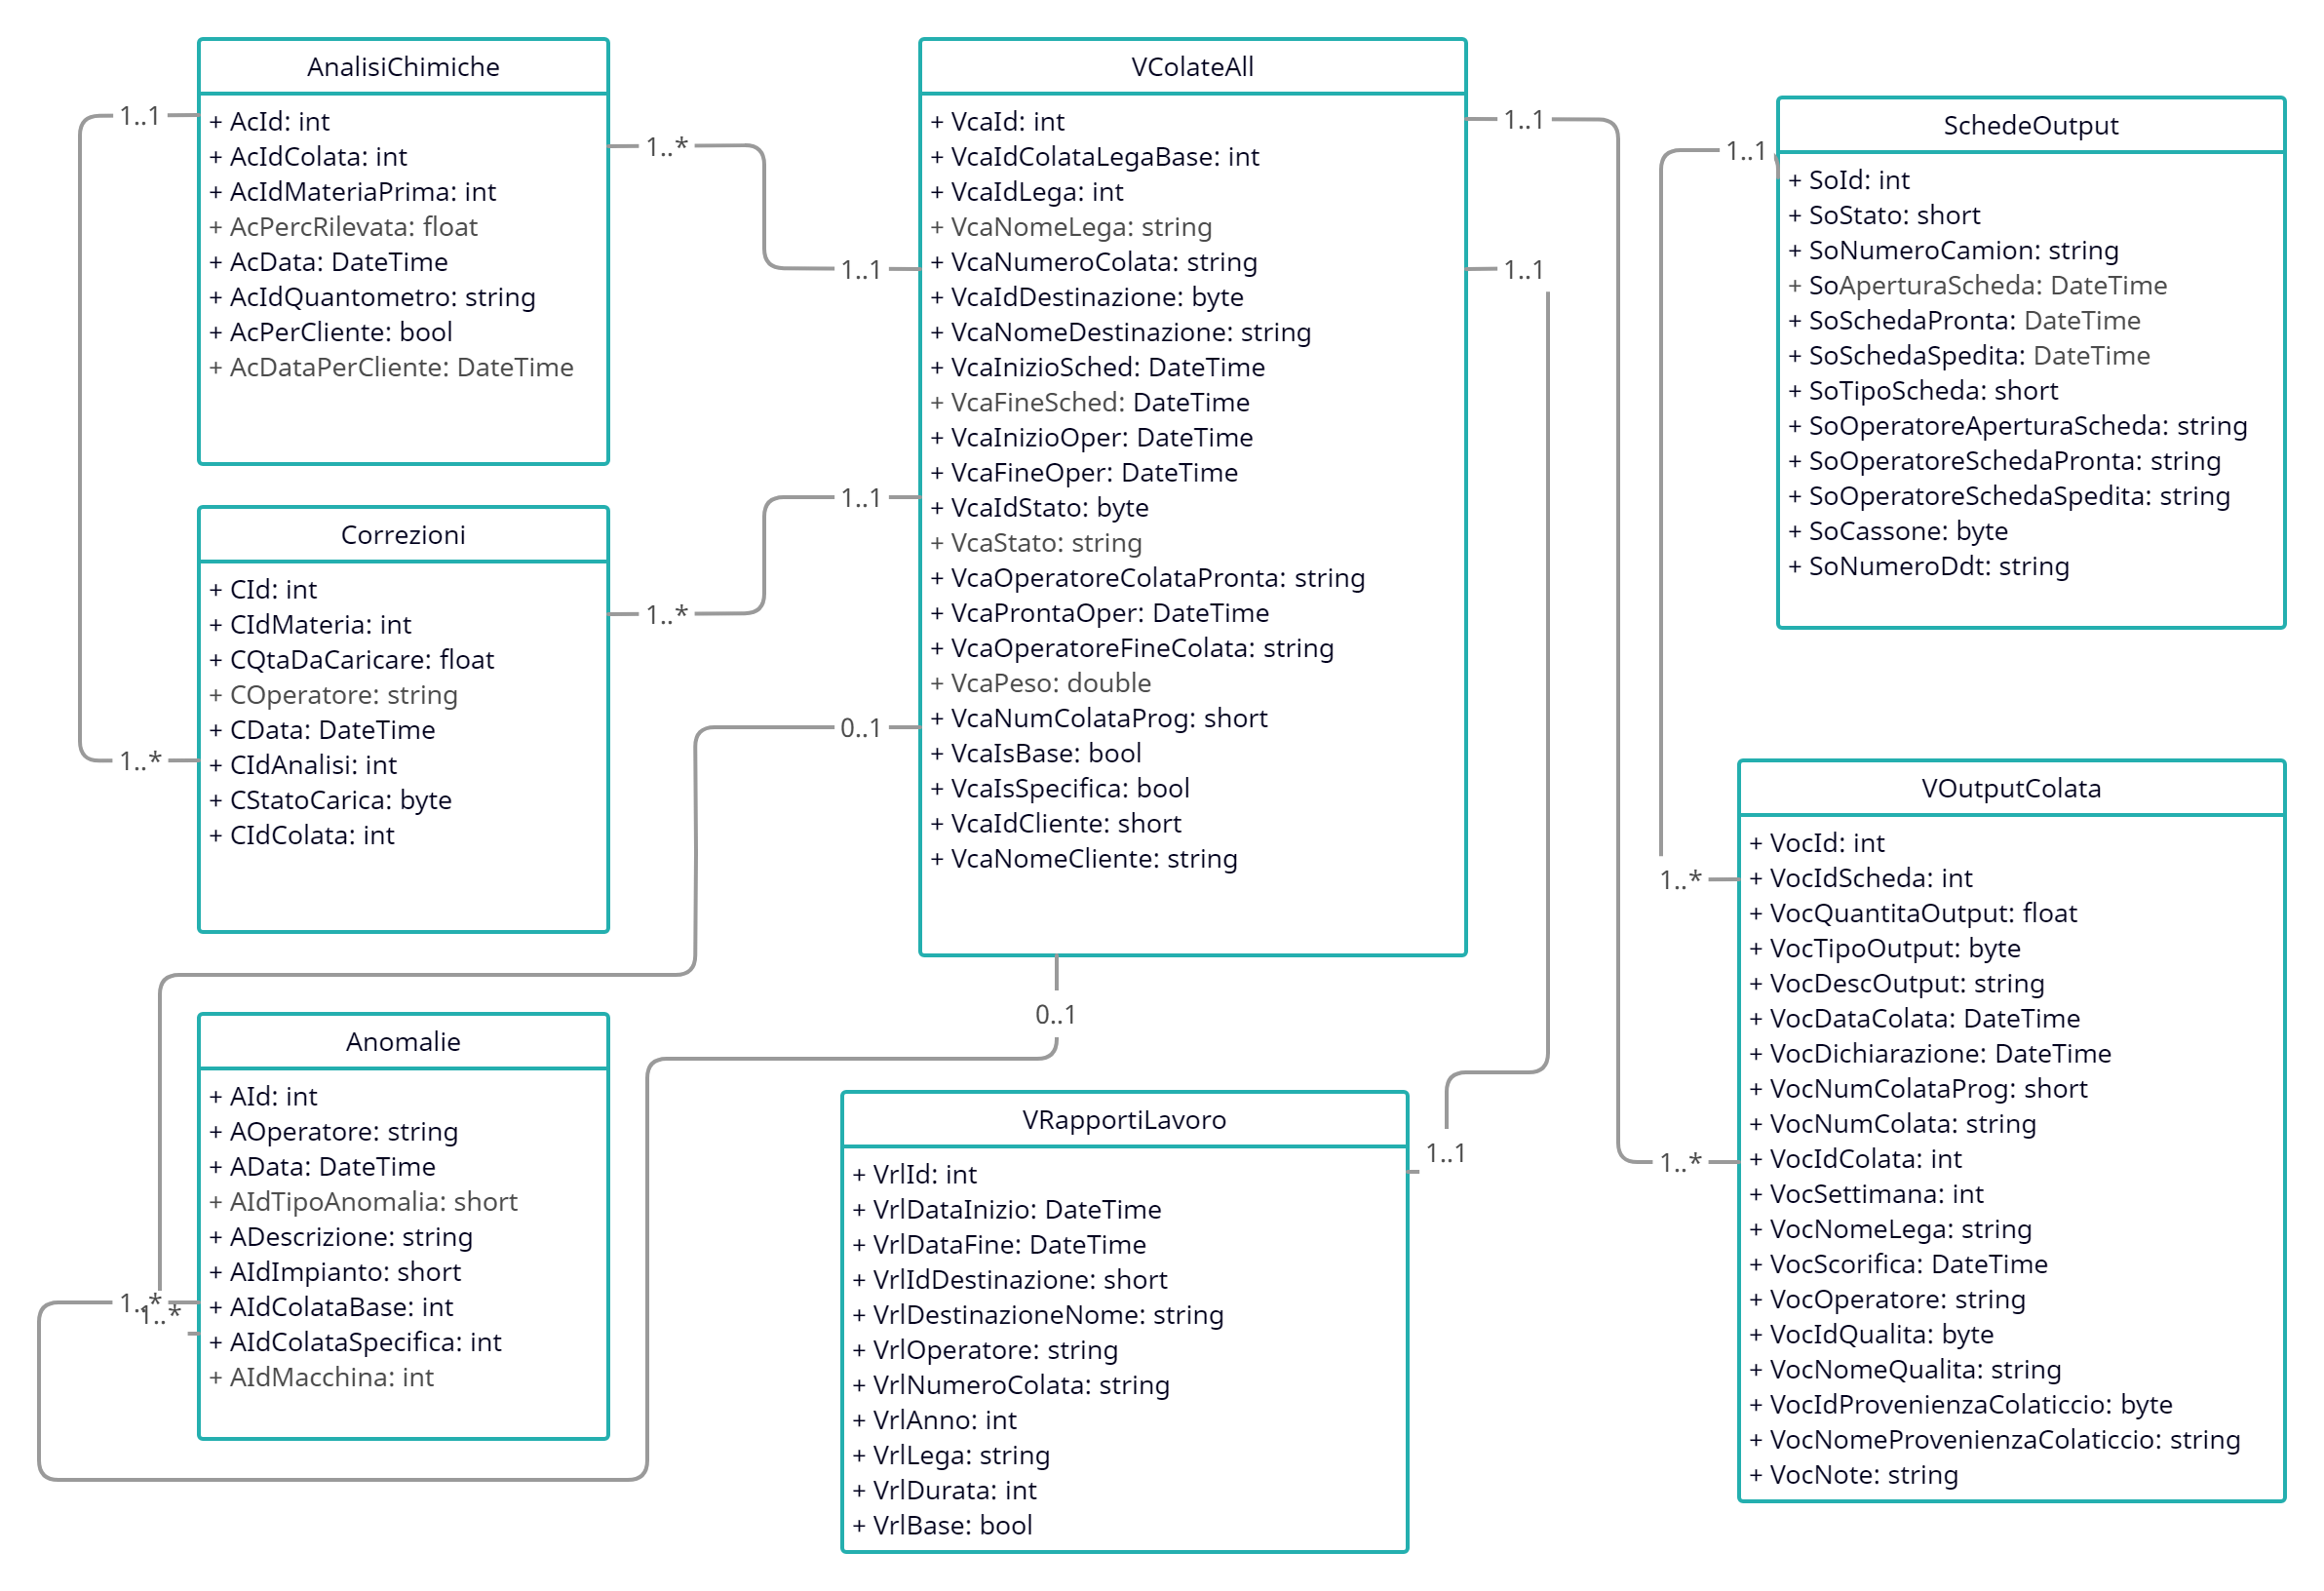
\includegraphics[width = \columnwidth]{ClassDiagram}
    \centering
    \caption{Diagramma delle classi}
    \label{fig:ClassDiagram}
  \end{figure}

  \subsection{AnalisiChimiche}
  La classe \textit{AnalisiChimiche} rappresenta il relativo oggetto nel database. Questo oggetto viene utilizzato per la
  rappresentazione delle rilevazioni delle Analisi Chimiche relative alle colate specifiche. Queste analisi chimiche vengono
  rilevate tramite uno strumento, chiamato quantometro, e memorizzate su dei file. Questi file vengono poi analizzati dalla
  web application \textit{Rapporti di Lavoro} e i dati relativi alle analisi chimiche vengono memorizzati nel database. I dati
  presenti in questo oggetto sono i seguenti:
  \begin{itemize}
    \item \textit{AcId}, ovvero l'identificativo progressivo dell'analisi chimica;
    \item \textit{AcIdColata}, ovvero il riferimento all'identificativo progressivo della colata a cui fa riferimento
    l'analisi;
    \item \textit{AcIdMateriaPrima}, ovvero il riferimento all'identificativo progressivo del materiale rilevato durante
    l'analisi;
    \item \textit{AcPercRilevata}, ovvero la quantità, in percentuale, dell'elemento rilevato presente all'interno della
    colata;
    \item \textit{AcData}, ovvero data e ora in cui è stata effettuata la rilevazione;
    \item \textit{AcIdQuantometro}, ovvero l'identificativo del quantometro, cioè lo strumento utilizzato per eseguire
    l'analisi chimica;
    \item \textit{AcPerCliente}, ovvero un flag che indica se l'analisi è l'analisi definita \textit{Per Cliente},
    ovvero l'analisi definitiva;
    \item \textit{AcDataPerCliente}, ovvero data e ora in cui è stata salvata l'analisi \textit{Per Cliente}.
  \end{itemize}

  \subsection{Anomalie}
  La classe \textit{Anomalie} rappresenta il relativo oggetto nel database. Questo oggetto viene utilizzato per la
  rappresentazione delle anomalie che si sono verificate durante una colata nei vari impianti. Nelle pagine relative
  ai rapporti di lavoro è presente una tabella che consente la visualizzazione di questi dati e la possibilità di aggiungere
  delle nuove anomalie tramite un popup che consente l'inserimento della data in cui l'anomalia si è verificata e 
  il tipo e la descrizione dell'anomalia. I dati presenti in questo oggetto sono i seguenti:
  \begin{itemize}
    \item \textit{AId}, ovvero l'identificativo progressivo dell'anomalia;
    \item \textit{AOperatore}, ovvero l'operatore che ha salvato l'anomalia;
    \item \textit{AData}, ovvero data e ora in cui si è verificata l'anomalia;
    \item \textit{AIdTipoAnomalia}, ovvero il riferimento all'identificativo progressivo del tipo di anomalia;
    \item \textit{ADescrizione}, ovvero eventuali note che l'operatore inserisce durante la fase di salvataggio dell'anomalia;
    \item \textit{AIdImpianto}, ovvero il riferimento all'identificativo dell'impianto in cui si è verificata l'anomalia;
    \item \textit{AIdColataBase}, ovvero il riferimento all'identificativo progressivo della colata base in corso
    nel momento in cui si è verificata l'anomalia;
    \item \textit{AIdColataSpecifica}, ovvero il riferimento all'identificativo progressivo della colata specifica
    in corso nel momento in cui si è verificata l'anomalia;
    \item \textit{AIdMacchina}, ovvero il riferimento all'identificativo progressivo della macchina nella quale
    si è verificata l'anomalia, utilizzato solo nei \textit{Rapporti Lavoro Colata Continua}.
  \end{itemize}
    
  \subsection{Colate}
  La classe \textit{VColateAll} rappresenta il relativo oggetto nel database. Questo oggetto viene utilizzato per la
  rappresentazione di tutte le informazioni relative alle colate (base e specifiche) che sono state schedulate. Queste
  informazioni vengono visualizzate nella pagina \textit{Storico Colate}. I dati presenti in questo oggetto sono i seguenti:
  \begin{itemize}
    \item \textit{VcaId}, ovvero l'identificativo progressivo della colata;
    \item \textit{VcaIdColataLegaBase}, ovvero il riferimento all'identificativo progressivo della colata base,
    utilizzato solo per le colate specifiche;
    \item \textit{VcaIdLega}, ovvero il riferimento all'identificativo della lega prodotta dalla colata;
    \item \textit{VcaNomeLega}, ovvero la descrizione relativa alla lega prodotta dalla colata;
    \item \textit{VcaNumeroColata}, ovvero il numero della colata;
    \item \textit{VcaIdDestinazione}, ovvero il riferimento all'impianto di destinazione della colata, cioè
    il forno verso il quale la colata base viene sversata;
    \item \textit{VcaNomeDestinazione}, ovvero il nome della destinazione della colata;
    \item \textit{VcaInizioSched}, ovvero data e ora prevista di inizio della colata;
    \item \textit{VcaFineSched}, ovvero data e ora prevista di fine della colata;
    \item \textit{VcaInizioOper}, ovvero data e ora effettive di inizio della colata;
    \item \textit{VcaFineOper}, ovvero data e ora effettive di fine colata;
    \item \textit{VcaIdStato}, ovvero il riferimento all'identificativo dello stato della colata;
    \item \textit{VcaStato}, ovvero la descrizione relativa allo stato della colata;
    \item \textit{VcaOperatoreColataPronta}, ovvero l'operatore che ha dichiarato la colata pronta;
    \item \textit{VcaProntaOper}, ovvero data e ora in cui la colata è stata dichiarata pronta;
    \item \textit{VcaOperatoreFineColata}, ovvero l'operatore che ha dichiarato la colata conclusa;
    \item \textit{VcaPeso}, ovvero il peso totale della colata;
    \item \textit{VcaNumColataProg}, ovvero il numero progressivo che identifica la colata, utilizzato solo per
    le colate specifiche;
    \item \textit{VcaIsBase}, ovvero un flag che indica se la colata è una colata base;
    \item \textit{VcaIsSpecifica}, ovvero un flag che indica se la colata è una colata specifica;
    \item \textit{VcaIdCliente}, ovvero il riferimento all'identificativo del cliente relativo alla colata;
    \item \textit{VcaNomeCliente}, ovvero il nome del cliente relativo alla colata.
  \end{itemize}
  
  \subsection{Correzioni}
  La classe \textit{Correzioni} rappresenta il relativo oggetto nel database. Questo oggetto viene utilizzato per la
  rappresentazione delle correzioni da effettuare alla colata in base ai calcoli effettuati sulle analisi chimiche.
  Nella pagina \textit{Analisi Chimiche} è infatti possibile effettuare i calcoli delle correzioni per le analisi chimiche
  che non rispettano la specifica. Quando queste proposte di correzioni vengono accettate, le rispettive informazioni vengono
  memorizzate tramite questo oggetto. I dati presenti in questo oggetto sono i seguenti:
  \begin{itemize}
      \item \textit{CId}, ovvero l'identificativo progressivo della correzione;
      \item \textit{CIdMateria}, ovvero il riferimento all'identificativo del correttivo che deve essere
      utilizzato per eseguire la correzione;
      \item \textit{CQtaDaCaricare}, ovvero la quantità del correttivo da caricare nella colata;
      \item \textit{COperatore}, ovvero il nome dell'operatore che ha accettato la correzione;
      \item \textit{CData}, ovvero data e ora in cui è stata accettata la proposta di correzione;
      \item \textit{CIdAnalisi}, ovvero il riferimento all'identificativo dell'analisi chimica di riferimento;
      \item \textit{CStatoCarica}, ovvero il riferimento all'identificativo dello stato carica della correzione;
      \item \textit{CIdColata}, ovvero il riferimento all'identificativo della colata della quale deve essere
      effettuata la correzione.
  \end{itemize}

  \subsection{Schede Output}
  La classe \textit{SchedeOutput} rappresenta il relativo oggetto nel database. Questo oggetto viene utilizzato per la
  rappresentazione delle schede contenenti le informazioni relative agli output delle varie colate. Ogni scheda equivale
  a un cassone presente in impianto che contiene tutti gli output relativi alle colate del relativo impianto. I dati
  presenti in questo oggetto sono i seguenti:
  \begin{itemize}
    \item \textit{SoId}, ovvero l'identificativo progressivo della scheda;
    \item \textit{SoStato}, ovvero il riferimento all'identificativo dello stato della scheda;
    \item \textit{SoNumeroCamion}, ovvero il progressivo del camion utilizzato per la spedizione del contenuto del
    cassone collegato alla scheda;
    \item \textit{SoAperturaScheda}, ovvero data e ora di apertura della scheda output;
    \item \textit{SoSchedaPronta}, ovvero data e ora di chiusura della scheda output;
    \item \textit{SoSchedaSpedita}, ovvero data e ora di spedizione della scheda output;
    \item \textit{SoTipoScheda}, ovvero il riferimento all'identificativo del tipo di scheda;
    \item \textit{SoOperatoreAperturaScheda}, ovvero l'operatore che ha aperto la scheda;
    \item \textit{SoOperatoreSchedaPronta}, ovvero l'operatore che ha dichiarato chiusa la scheda;
    \item \textit{SoOperatoreSchedaSpedita}, ovvero l'operatore che ha dichiarato la spedizione della scheda;
    \item \textit{SoCassone}, ovvero il riferimento all'identificativo progressivo del cassone di riferimento;
    \item \textit{SoNumeroDdt}, ovvero il numero del documento di trasporto (\textit{DDT}) relativo alla spedizione
    della scheda.
  \end{itemize}

  \subsection{Output Colata}
  La classe \textit{VOutputColata} rappresenta il relativo oggetto nel database. Questo oggetto viene utilizzato per la
  rappresentazione delle informazioni relative agli output di tutte le colate, base e specifiche. I dati presenti in questo
  oggetto sono i seguenti:
  \begin{itemize}
    \item \textit{VocId}, ovvero l'identificativo progressivo dell'output della colata;
    \item \textit{VocIdScheda}, ovvero il riferimento all'identificativo della scheda in cui è memorizzato l'output;
    \item \textit{VocQuantitaOutput}, ovvero la quantità totale dell'output;
    \item \textit{VocTipoOutput}, ovvero l'identificativo del tipo di output;
    \item \textit{VocDescOutput}, ovvero il descrittivo del tipo di output;
    \item \textit{VocDataColata}, ovvero data e ora di inizio della colata;
    \item \textit{VocDichiarazione}, ovvero data e ora in cui è stato inserito l'output;
    \item \textit{VocNumColataProg}, ovvero il numero progressivo della colata di riferimento;
    \item \textit{VocNumColata}, ovvero il numero della colata di riferimento;
    \item \textit{VocIdColata}, ovvero il riferimento all'id della colata relativa;
    \item \textit{VocSettimana}, ovvero il numero della settimana nell'anno in cui è stata effettuata la scorifica;
    \item \textit{VocNomeLega}, ovvero il nome della lega relativa alla colata di riferimento;
    \item \textit{VocScorifica}, ovvero data e ora in cui è stata effettuata la scorifica;
    \item \textit{VocOperatore}, ovvero l'operatore che ha inserito l'output;
    \item \textit{VocIdQualita}, ovvero il riferimento all'id della qualità dell'output;
    \item \textit{VocNomeQualita}, ovvero il descrittivo della qualità dell'output;
    \item \textit{VocIdProvenienzaColaticcio}, ovvero il riferimento all'id della provenienza dell'output;
    \item \textit{VocNomeProvenienzaColaticcio}, ovvero il descrittivo della provenienza dell'output;
    \item \textit{VocNote}, ovvero eventuali note inserite dall'operatore che ha aggiunto l'output.
  \end{itemize}
  

  \subsection{Rapporti Lavoro}
  La classe \textit{VRapportiLavoro} rappresenta il relativo oggetto nel database. Questo oggetto viene utilizzato per la
  rappresentazione delle informazioni relative ai rapporti di lavoro visualizzate nelle rispettive pagine.
  Questo oggetto rappresenta sia i rapporti di lavoro relativi alle colate base utilizzati nei rapporti di lavoro del forno
  fusorio, sia i rapporti di lavoro relativi alle colate specifiche utilizzati nei rapporti di lavoro dei forni bacino, della
  colata continua e del magazzino pani. I dati presenti in questo oggetto sono i seguenti:
  \begin{itemize}
    \item \textit{VrlId}, ovvero l'identificativo progressivo della colata di riferimento;
    \item \textit{VrlDataInizio}, ovvero data e ora di inizio della colata di riferimento;
    \item \textit{VrlDataFine}, ovvero data e ora di fine della colata di riferimento;
    \item \textit{VrlIdDestinazione}, ovvero il riferimento all'identificativo della destinazione della colata;
    \item \textit{VrlDestinazioneNome}, ovvero il descrittivo della destinazione di riferimento;
    \item \textit{VrlOperatore}, ovvero l'operatore che ha dato inizio alla colata;
    \item \textit{VrlNumeroColata}, ovvero il numero della colata di riferimento;
    \item \textit{VrlAnno}, ovvero l'anno in cui la colata è stata prodotta;
    \item \textit{VrlLega}, ovvero la lega prodotta dalla colata di riferimento;
    \item \textit{VrlDurata}, ovvero la durata della colata di riferimento;
    \item \textit{VrlBase}, ovvero un flag che indica se il rapporto fa riferimento a una colata base o specifica;
  \end{itemize}
  
  
  \section{Controller}
  All'interno di questo paragrafo vengono illustrati i controller utilizzati nella web application \textit{Rapporti di Lavoro}
  e i relativi metodi più importanti.

  \subsection{AnalisiChimicheController}
  La classe \textit{AnalisiChimicheController} contiene tutte le funzioni relative alle Analisi Chimiche, come le funzioni per
  il calcolo delle correzioni o per il salvataggio delle proposte di correzioni. I metodi più significativi di questa classe
  sono i seguenti:
  \begin{itemize}
    \item \textit{AnalisiFile}. Questo metodo viene eseguito ogni minuto e analizza i file csv memorizzati in una determinata
    cartella (il quale percorso è configurabile). Questi file vengono analizzati per memorizzare nel database i dettagli
    dell'analisi chimica che ha generato il file stesso. I dati letti nel file e salvati nel database sono
    l'id del quantometro, il numero della colata, il tipo di analisi, l'id dell'elemento chimico e la percentuale rilevata.
    Inoltre, se l'elemento chimico non è presente nel relativo dizionario, questo viene aggiunto in automatico con dati
    impostati di default, poi modificabili dalla sezione \textit{Materie e Elementi};
    \item \textit{GetChemicalForColata}. Questo metodo prende come parametro l'id e la destinazione della colata della
    quale ottenere la lista delle relative analisi chimiche da visualizzare nella pagina \textit{Analisi Chimiche}.
    Il metodo restituisce un array contenente tutti i dati letti dal database, di tutte le analisi chimiche relative alla
    colata passata come parametro;
    \item \textit{GetElencoAnalisi}. Questo metodo prende come parametri l'id dell'impianto, l'id e il peso della colata e
    l'id dell'analisi desiderata e restituisce i relativi dettagli, come l'elemento, la percentuale rilevata, il peso
    (calcolato in base alla percentuale e al peso totale della colata) e le specifiche da rispettare per rimanere
    all'interno dello standard. Il metodo restituisce un oggetto contenente i dettagli dell'analisi e delle
    correzioni eventualente già accettate e memorizzate nel database;
    \item \textit{CalcoloPropostaCorrezioni}. Questo metodo prende come parametri l'elenco delle rilevazioni relative a
    un'analisi chimica e restituisce un oggetto contenente le proposte di correzione per quella determinata analisi chimica.
    In questo metodo vengono calcolate le quantità dei correttivi da utilizzare per adattare le quantità degli
    elementi chimici agli standard produttivi.
  \end{itemize}

  \subsection{ColateController}
  La classe \textit{ColateController} contiene tutte le funzioni relative alle colate, come le funzioni per la lettura delle
  colate attualmente in corso o l'inserimento di nuove informazioni relative alla colata. I metodi più significativi
  di questa classe sono i seguenti:
  \begin{itemize}
    \item \textit{GetActualColataFornoFusorio}. Questo metodo restituisce un oggetto di tipo \textit{VColateAll}
    contenente le informazioni relative alla colata attualmente in corso nel Forno Fusorio;
    \item \textit{GetActualColataForniBacino}. Questo metodo restituisce un oggetto di tipo \textit{VColateAll}
    contenente le informazioni relative alla colata attualmente in corso nel Forno a Bacino passato come parametro al metodo;
    \item \textit{AddPesoColata}. Questo metodo consente di salvare nel database il peso totale della colata passata
    come parametro;
    \item \textit{GetColateBaseByDate}. Questo metodo restituisce un array di oggetti conteneti le informazioni relative
    alle colate base con data di inizio o di schedulazione compresa tra le date di inizio e di fine passate come parametro;
    \item \textit{GetColateSpecificheByBase}. Questo metodo restituisce un array di oggetti contenenti le informazioni
    relative alle colate specifiche che fanno riferimento alla colata base passata come parametro;
    \item \textit{GetLegheBaseByColata}. Questo metodo restituisce le informazioni della lega base relativa alla
    colata base passata come parametro;
    \item \textit{GetLegheSpecificheByColata}. Questo metodo restituisce le informazioni della lega specificha relativa
    alla colata specifica passata come parametro.
  \end{itemize}

  \subsection{OuptutColataController}
  \begin{itemize}
    \item \textit{AddOutputBase}. Questo metodo inserisce nel database la registrazione dell'output di una colata base
    passato come parametro;
    \item \textit{MoveOutputBase}. Questo metodo cambia il riferimento di una registrazione di un output base da una
    scheda output a un'altra scheda passata come parametro;
    \item \textit{AddOutputSpecifica}. Questo metodo inserisce nel database la registrazione dell'output di una colata
    specifica passato come parametro;
    \item \textit{MoveOutputSpecifica}. Questo metodo cambia il riferimento di una registrazione di un output specifico
    da una scheda output a un'altra scheda passata come parametro;
    \item \textit{GetOutputColataBaseByScheda}. Questo metodo restituisce gli output base che fanno riferimento alla
    scheda passata come parametro;
    \item \textit{GetOutputColataSpecificaByScheda}. Questo metodo restituisce gli output specifici che fanno riferimento alla
    scheda passata come parametro;
  \end{itemize}

  \subsection{RapportiDiLavoroController}
  \begin{itemize}
    \item \textit{GetRapportoFornoFusorioActualColata}. Questo metodo restituisce il rapporto di lavoro base in
    corso attualmente;
    \item \textit{GetRapportoForniBacinoActualColata}. Questo metodo restituisce il rapporto di lavoro relativa alla
    colata attualmente in corso nel forno a bacino passato come parametro;
    \item \textit{GetRapportoColataContinuaActualColata}. Questo metodo restituisce il rapporto di lavoro relativa
    alla colata attualmente in corso nella colata continua;
    \item \textit{GetRapportiColataContinuaByYear}. Questo metodo restituisce l'elenco di tutti i rapporti specifici
    della colata continua ordinati per data in modo decrescente e filtrati in base all'anno passato come parametro;
    \item \textit{GetRapportiMagazzinoPaniByYear}. Questo metodo restituisce l'elenco di tutti i rapporti specifici
    del magazzino pani ordinati per data in modo decrescente e filtrati in base all'anno passato come parametro;
    \item \textit{GetFermiFornoFusorio}. Questo metodo restituisce la lista di fermi che si sono verificati
    all'interno del turno passato come parametro;
    \item \textit{GetFermiColataContinuaByColata}. Questo metodo restituisce la lista di fermi che si sono
    verificati durante la colata passata come parametro;
    \item \textit{GetFermiMagazzinoPaniByColata}. Questo metodo restituisce la lista di fermi che si sono
    verificati durante la colata passata come parametro;
    \item \textit{AddFermo}. Questo metodo consente di aggiungere un nuovo fermo manualmente, con data e ora
    di inizio e di fine e i cinque perchè passati come parametro;
    \item \textit{EditListaFermo}. Questo metodo consente di modificare il fermo passato come parametro e viene
    metodo viene utilizzato per causalizzate i fermi automatici salvati dal PLC;
    \item \textit{AddAnomalia}. Questo metodo consente di inserire nel database una nuova anomalia che viene
    passata come parametro;
    \item \textit{GetAnomalieFornoFusorioByShift}. Questo metodo restituisce l'elenco di anomalie che si sono
    verificate nel forno fusorio durante il turno passato come parametro;
    \item \textit{GetAnomalieColataContinuaByColata}. Questo metodo restituisce l'elenco di anomalie che si sono
    verificate nel reparto di colata continua durante la colata passata come parametro;
    \item \textit{GetAnomalieMagazzinoPaniByColata}. Questo metodo restituisce l'elenco di anomalie che si sono
    verificate nel reparto magazzino pani durante la colata passata come parametro;
    \item \textit{GetAnomalieForniBacinoByColata}. Questo metodo restituisce l'elenco di anomalie che si sono
    verificate nel forno a bacino durante la colata e nel forno passati come parametro;
    \item \textit{AddRallentamento}. Questo metodo consente di inserire nel database un nuovo rallentamento che
    viene passato come parametro;
    \item \textit{GetRallentamentiColataContinua}. Questo metodo restituisce l'elenco di rallentamenti che si sono
    verificati nel reparto di colata continua durante la colata passata come parametro;
    \item \textit{GetNoteFornoFusorioByShift}. Questo metodo restituisce l'elenco di note relative al forno fusorio che
    sono state inserite durante il turno passato come parametro;
    \item \textit{GetNoteColataContinuaActualColata}. Questo metodo restituisce l'elenco di note relative alla colata
    continua che sono state inserite durante la colata passata come parametro;
    \item \textit{GetNoteColataContinuaPrevTenColate}. Questo metodo restituisce l'elenco di note relative alla colata
    continua che sono state inserite durante le ultime dieci colate precedenti a quella passata come parametro;
    \item \textit{GetNoteMagazzinoPaniActualColata}. Questo metodo restituisce l'elenco di note relative al magazzino
    pani che sono state inserite durante la colata passata come parametro;
    \item \textit{GetNoteMagazzinoPaniPrevTenColate}. Questo metodo restituisce l'elenco di note relative al magazzino
    pani che sono state inserite durante le ultime dieci colate passate come parametro;
    \item \textit{GetNoteForniBacinoByShift}. Questo metodo restituisce l'elenco di note relative al forno bacino che
    sono state inserite durante il turno passato e nel forno passati come parametro;
    \item \textit{AddNota}. Questo metodo consente di inserire una nuova nota per il reparto passato come parametro;
    \item \textit{GetPassaggioConsegneColataContinua}. Questo metodo restituisce l'elenco di passaggi di consegne
    relative alla colata continua che sono stati inseriti durante la colata passata come parametro;
    \item \textit{GetPassaggioConsegneMagazzinoPani}. Questo metodo restituisce l'elenco di passaggi di consegne
    relative al magazzino pani che sono stati inseriti durante la colata passata come parametro;
    \item \textit{GetPassaggioConsegneColataContinuaPrevShift}. Questo metodo restituisce l'elenco di passaggi di
    consegne relative alla colata continua che sono stati inseriti durante il turno precedente a quello attuale,
    passato come parametro;
    \item \textit{GetPassaggioConsegneMagazzinoPaniPrevShift}. Questo metodo restituisce l'elenco di passaggi di
    consegne relative al magazzino pani che sono stati inseriti durante il turno precedente a quello attuale,
    passato come parametro;
    \item \textit{GetPaniDaRifondereListByColata}. Questo metodo restituisce l'elenco delle rilevazioni dei pani da
    rifondere che sono state inserite durante la colata passata come parametro;
    \item \textit{AddPaniDaRifondere}. Questo metodo consente di inserire una nuova rilevazione di pani da rifondere
    che viene passata come parametra;
    \item \textit{GetInterruzioniMagazzinoPani}. Questo metodo restituisce l'elenco di interruzioni verificatesi nel
    magazzino pani relative alla colata passata come parametro;
    \item \textit{AddInterruzione}. Questo metodo consente di inserire una nuova interruzione all'orario passato come
    parametro;
    \item \textit{CloseInterruzione}. Questo metodo consente di chiudere l'interruzione in corso impostando come
    orario di fine quello passato come parametro;
    \item \textit{GetNumeroFormatoPacchi}. Questo metodo restituisce il numero e il formato dei pacchi che vengono
    analizzati nel reparto magazzino pani. Il metodo viene richiamato ogni minuto e interroga un servizio esterno chiamato
    WorkerMsgScadaService, sempre sviluppato dal team di \textit{Adipso}, per ricevere le informazioni direttamente dal
    server SCADA;
    \item \textit{GetTempiComponenti}. Questo metodo restituisce le informazioni sul tempo di lavoro dei componenti
    nel reparto di colata continua. Il metodo viene richiamato ogni dieci minuti e interroga il servizio esterno
    WorkerMsgScadaService per ricevere le informazioni direttamente dal server SCADA;
    \item \textit{ResetOreLavoro}. Questo metodo consente di resettare le informazioni sul tempo di lavoro dei
    componenti nel reparto di colata continua. Il metodo invia al servizio esterno WorkerMsgScadaService la richiesta
    di reset dei tag e restituisce l'esito dell'operazione.
  \end{itemize}



  \subsection{SchedeOutputController}
  \begin{itemize}
    \item \textit{AddNewScheda}. Questo metodo consente di creare una nuova scheda associata a un determinato cassone.
    Questo metodo viene richiamato in automatico ogni volta che una scheda viene chiusa, per creare una nuova scheda
    relativa allo stesso cassone di quella precedente. Inoltre questo metodo viene richiamato anche su richiesta
    dell'utente per inserire una nuova scheda solo per un cassone che non ha alcuna scheda associata;
    \item \textit{CloseScheda}. Questo metodo consente di chiudere la scheda passata come parametro e di dichiarla
    \textit{IN ATTESA DI SPEDIZIONE};
    \item \textit{AddNCamion}. Questo metodo consente di dichiarare una scheda come spedita e a inserire il numero
    progressivo del camion che ha spedito la scheda;
    \item \textit{AddNDdt}. Questo metodo consente di inserire le informazioni relative al documento di trasporto
    associato alla spedizione di una determinata scheda output passata come parametro;
    \item \textit{GetSchedaAttivaByCassone}. Questo metodo restituisce le informazioni relative alla scheda
    attualmente aperta relativa la cassone passato come parametro;
    \item \textit{GetSchedeBaseChiuseByDate}. Questo metodo restituisce l'elenco di tutte le schede base chiuse
    comprese nel periodo di tempo passate come parametro;
    \item \textit{GetSchedeBaseAperte}. Questo metodo restituisce le informazioni relative a tutte le schede base aperte;
    \item \textit{GetSchedeSpecificheChiuseByDate}. Questo metodo restituisce l'elenco di tutte le schede specifiche
    chiuse comprese nel periodo di tempo passate come parametro;
    \item \textit{GetSchedeSpecificheAperte}. Questo metodo restituisce le informazioni relative a tutte le schede
    specifiche aperte;
    \item \textit{GetSchedaById}. Questo metodo restituisce le informazioni relative alla scheda che ha come
    identificativo il valore passato come parametro.
  \end{itemize}



  \subsection{ShiftController}
  \begin{itemize}
    \item \textit{GetActualShift}. Questo metodo restituisce le informazioni relative al turno in corso in base
    all'utente passato come parametro e al tipo di turno dello stesso utente. Le informazioni restituite sono
    la data di inizio, di fine e il numero del turno nella giornata;
    \item \textit{GetPreviousShift}. Questo metodo restituisce le informazioni relative al turno precedente a
    quello attuale base all'utente passato come parametro e al tipo di turno dello stesso utente. Le informazioni
    restituite sono la data di inizio, di fine e il numero del turno nella giornata;
    \item \textit{GetOperatoriASupporto}. Questo metodo restituisce l'elenco degli operatori a supporto dell'operatore
    principale nell'impianto e nel turno passati come parametro.
  \end{itemize}

  \subsection{UserController}
  \begin{itemize}
    \item \textit{AuthenticateSupportUser}. Questo metodo consente di effettuare il login degli operatori di supporto,
    ovvero operatori che assistono gli operatori primari nei diversi reparti;
    \item \textit{AuthenticateUser}. Questo metodo consente di effettuare il login degli operatori che viene effettuato
    all'apertura della web application. Il login viene effettuato in base alla tipologia di security impostata nel
    file di configurazione. Di default è impostata la tipologia \textit{Domain}, quindi le credenziali da inserire
    durante la fase di login sono legate al dominio a cui appartiene il server sul quale è installata la web application;
    \item \textit{LoadAllFunctByUserGroup}. Questo il metodo viene utilizzato per recuperare dal database le funzionalità
    a cui ha accesso un determinato utente in base al suo gruppo di appartenenza, che viene passato come parametro.    
  \end{itemize}